\documentclass[12pt]{article}
\usepackage{fancyhdr,nameref}
\usepackage[a4paper,margin=1cm,top=1in,footskip=0.5cm]{geometry}
\usepackage{enumitem}
\usepackage{listings}
\usepackage{courier,caption,soul}
\usepackage{amsmath,amsfonts,fixmath}
\usepackage{tabu,array,graphicx}
\usepackage[nodayofweek]{datetime}
\usepackage[usenames,dvipsnames]{xcolor}
\usepackage{pgfplots}
\usepackage{circuitikz,siunitx}
\usepackage{titlesec}
\usepackage{tabto}
\usepackage[absolute]{textpos}
\usepackage{pdflscape}
\usepackage{pdfpages}
\usepackage{makecell}
\usepackage{multirow}
\pgfplotsset{compat=1.12}
\everymath{\displaystyle}
\setlength\extrarowheight{4pt}
\newdateformat{datef}{\twodigit{\THEDAY}{ }\shortmonthname[\THEMONTH]{ }\THEYEAR}
\newdate{date}{17}{07}{2015} % parameters are DDMMMYYYY format; output is DD MMM YYYY format
\pagestyle{fancy}
\fancyhf{}
\fancyhf[FC]{\thepage}
\fancyhf[HL]{\slshape COSC 2203-01}
\fancyhf[HC]{\scshape Component A}
\fancyhf[HR]{\slshape \leftmark}
\newcommand{\hlc}[2][yellow]{ {\sethlcolor{#1} \hl{#2}} }
\newcommand{\hlbox}[1]{\colorbox{cyan!50}{#1}}
\newcommand{\qw}[1]{\si{.#1}}
%\titleformat*{\section}{\LARGE\bfseries\ttfamily}
\definecolor{dkgreen}{RGB}{0,102,0}
\definecolor{gray}{rgb}{0.5,0.5,0.5}
\definecolor{mauve}{rgb}{0.58,0,0.82}
\lstset{frame=tb,
	escapeinside={\%*}{*)},
	captionpos=t,
	language=Java,
	aboveskip=3mm,
	belowskip=3mm,
	showstringspaces=false,
	columns=flexible,
	basicstyle={\small\ttfamily},
	numbers=none,
	numbersep=0pt,
	numberstyle=\small\ttfamily\color{gray},
	keywordstyle=\color{blue},
	commentstyle=\color{dkgreen},
	stringstyle=\color{mauve},
	breaklines=true,
	breakatwhitespace=true,
	tabsize=3}
\begin{document}
\newcolumntype{C}{>{\centering\arraybackslash}p{1em}}
	
	\begin{titlepage}
\newcommand{\HRule}{\rule{\linewidth}{0.5mm}} % Defines a new command for the horizontal lines, change thickness here

\center % Center everything on the page
 
%----------------------------------------------------------------------------------------
%	HEADING SECTIONS
%----------------------------------------------------------------------------------------

\textsc{\LARGE LeTourneau University}\\[1.0cm] % Name of your university/college
\textsc{\Large COSC 2203-01}\\[0.5cm] % Major heading such as course name
\textsc{\large Data Structures}\\[0.5cm] % Minor heading such as course title

%----------------------------------------------------------------------------------------
%	TITLE SECTION
%----------------------------------------------------------------------------------------

\HRule \\[0.4cm]
{ \huge \bfseries Programming Assignment \#4\\Component A}\\[0.2cm] % Title of your document
\HRule \\[1.5cm]
 
%----------------------------------------------------------------------------------------
%	Problem Set Section
%----------------------------------------------------------------------------------------

{\Large\bfseries ``Project Feasibility''}\\[5mm]
{\Large \emph{Using weighted digraphs}} \\[1.5cm]


%----------------------------------------------------------------------------------------
%	AUTHOR SECTION
%----------------------------------------------------------------------------------------
\begin{minipage}{0.35\textwidth}
	\begin{flushleft} \large
		\emph{Author:}\\
		Brian \textsc{Scott} % My name
	\end{flushleft}
\end{minipage}
~
\begin{minipage}{0.35\textwidth}
	\begin{flushright} \large
		\emph{Presented to:} \\
		Dr. Brent \textsc{Baas} % Supervisor's Name
	\end{flushright}
\end{minipage}\\[4cm]

%----------------------------------------------------------------------------------------
%	DATE SECTION
%----------------------------------------------------------------------------------------

{\large \datef\displaydate{date}}\\[2cm] % Date, change the \today to a set date if you want to be precise

%----------------------------------------------------------------------------------------
%	LOGO SECTION
%----------------------------------------------------------------------------------------
\vfill % Fill the rest of the page with whitespace

\includegraphics[scale=0.20]{gfx/logoHoriz.jpg}\\[1cm] % Include a department/university logo - this will require the graphicx package
 
%----------------------------------------------------------------------------------------

\end{titlepage}
	\section{Problem Description}
	This program analyzes a project, represented as an activity-on-edge digraph, and reports various statistics describing the project. The program makes use of a weighted graph to represent the inter-dependencies among the activities in the given project.
	
	\section{Input / Output Analysis}
	\subsection{Input}
	The input will be in the form of a text file, the project description, which will be fed through standard input. The first line of the input is equal to the number of stages in the project; each successive line contains the stage number, the number of adjacent stages, and a set of pairs. The pairs describe an adjacent stage number and it's activity cost, respectively.
	
	\begin{lstlisting}[caption=Sample input]
		5
		1 2 2 6 3 9
		2 1 4 2
		3 3 2 3 4 6 5 8
		4 1 5 1
		5 0
	\end{lstlisting}
	\subsection{Output}
	The output of the program is a text file containing the following information describing the project:
	\begin{itemize}
		\item Whether or not the project is feasible
		\item A linear ordering of the project activities (topological order)
		\item The early and late times of each stage in the project
		\item The total time required to complete the project
		\item The early and late times of each activity in the project
		\item A listing of the project's critical activities
	\end{itemize}
	The output filename will be in the format ``\texttt{\emph{<input\_filename>}.rpt.txt}''.
	\newpage
	\begin{lstlisting}[caption=Sample output]
		Project is feasible
		
		Ordering: 1 3 2 4 5
		
		Stg. Early Late
		1 	  		0 			0
		2 	  		12 		14
		3 	  		9 			9
		4 	  		15 		16
		5 	  		17 		17
		
		Total Project Time: 17
		
		Act.	 Early	 Late
		1 		   0 	 		8
		2 		   0 	 		0
		3 		   12 	 	14
		4 		   9 	 		11
		5 	 	   9 	 		10
		6 		   9 	 		9
		7 		   15 	 	16
		
		Critical Activities: 2, 6
	\end{lstlisting}
	\newpage
	
	\section{Program Design}
	\subsection{Class Diagram}
	\begin{center}
		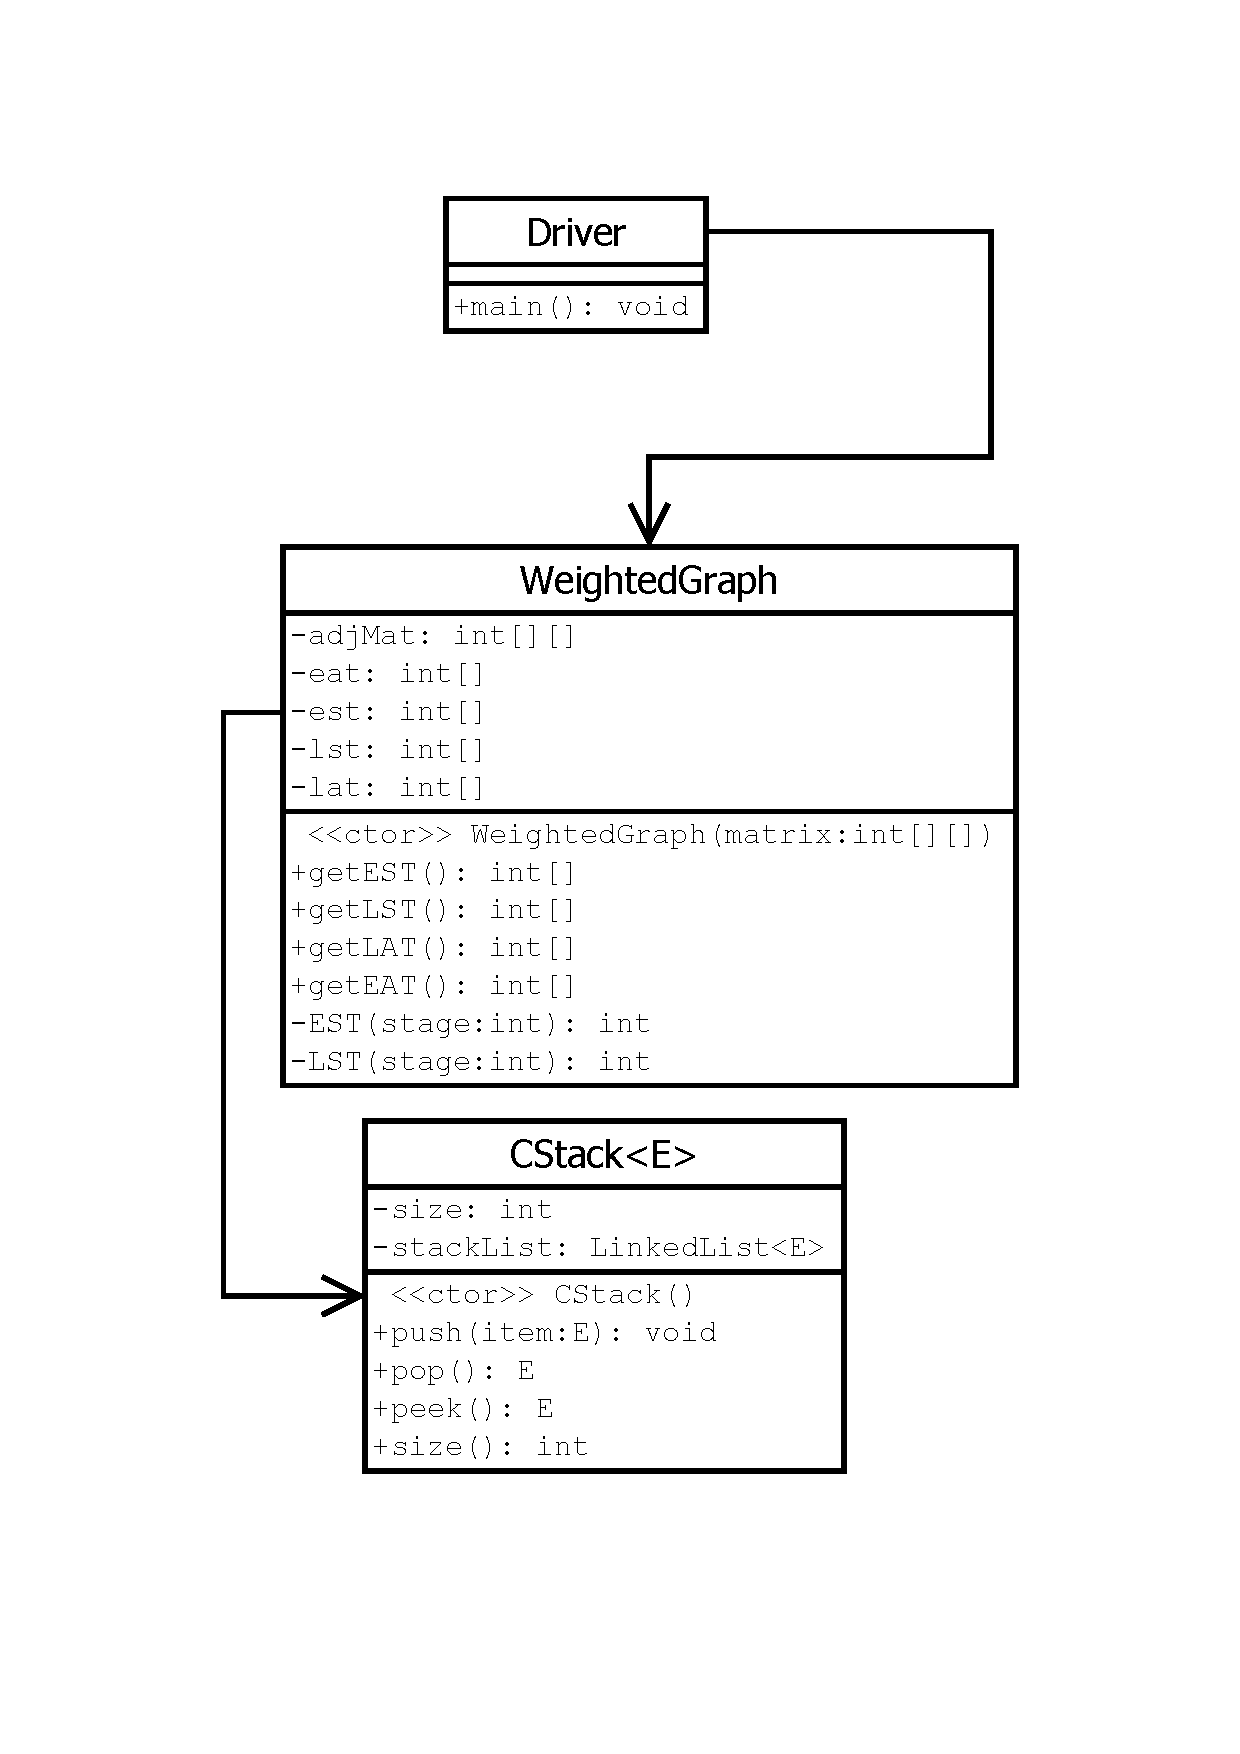
\includegraphics[scale=0.80]{4/cd.pdf}
	\end{center}
	\newpage
	\thispagestyle{empty}
	\begin{landscape}
		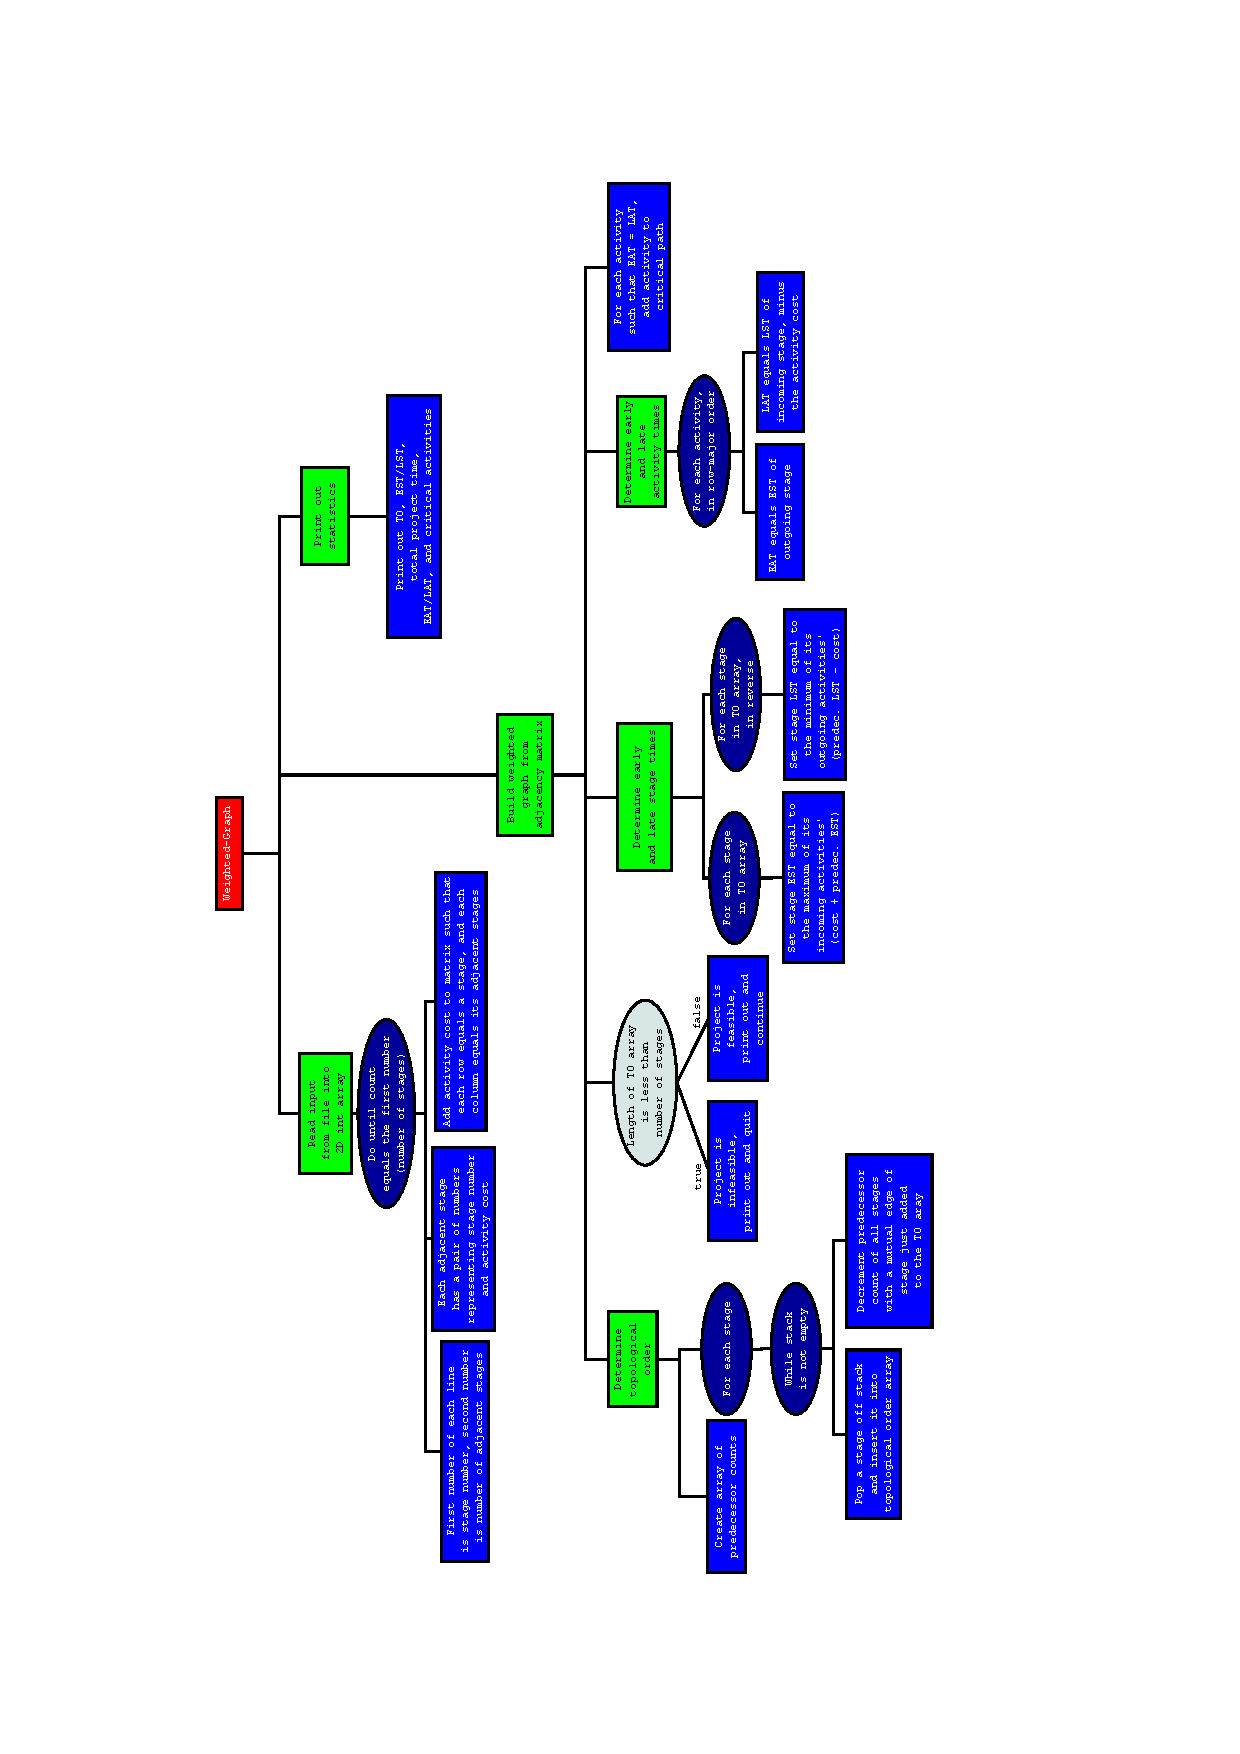
\includepdf[pages={1},scale=1.23,pagecommand=\subsection{Design Chart}]{4/deschart.pdf}
	\end{landscape}


	\section{Data Structure Graphics}
	\subsection{Weighted Directed Graph:}
	\begin{center}
		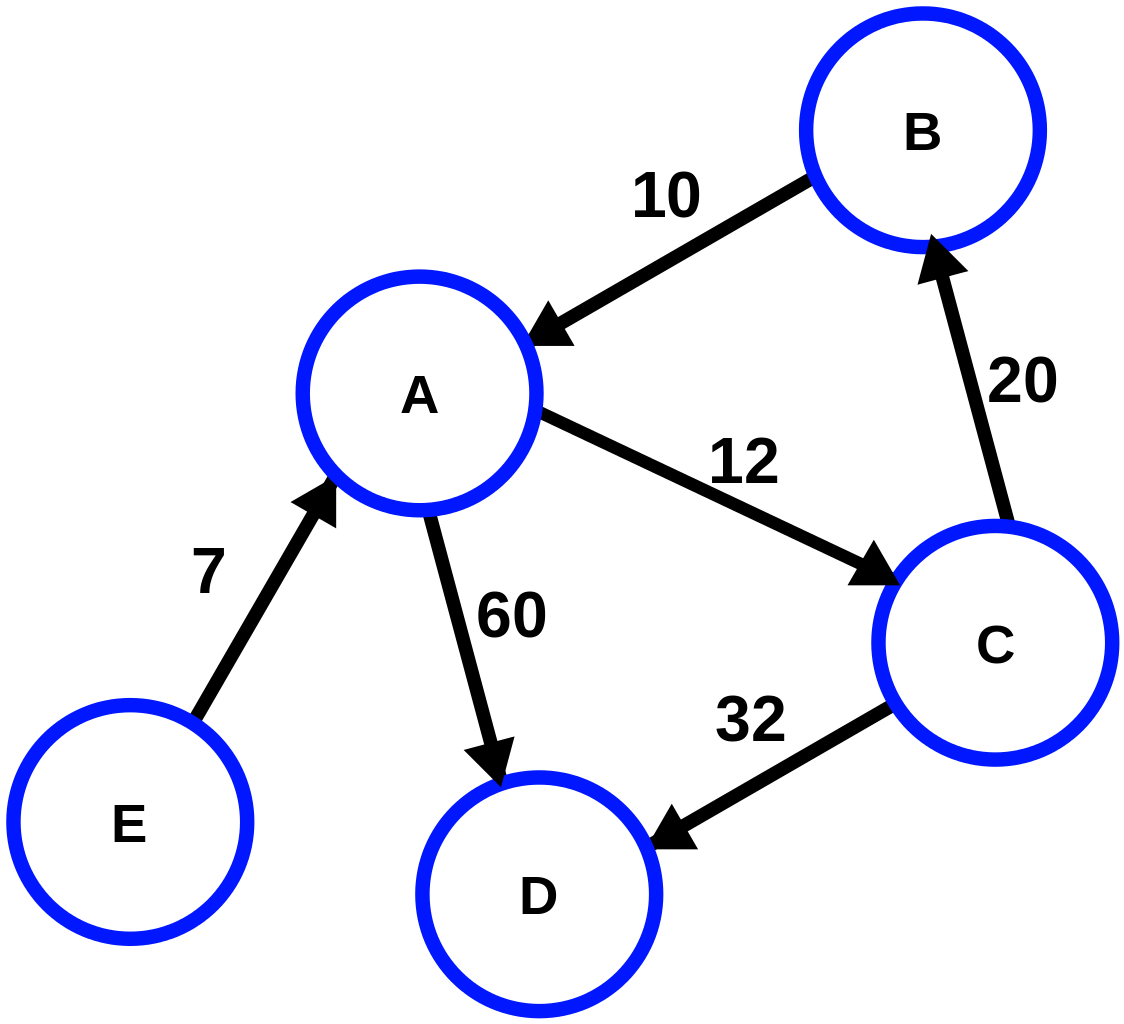
\includegraphics[scale=0.2]{4/weighted_graph.png}
	\end{center}
	\subsection{Adjacency Matrix:}
	\begin{center}
		\emph{Correlates to the above graph} \\[5mm]
		$\begin{pmatrix}
			  & A & B & C & D & E\\
			A & - & 0 & 12 & 60 & 0\\
			B & 10 & - & 0 & 0 & 0\\
			C & 0 & 20 & - & 32 & 0\\
			D & 0 & 0 & 0 & - & 0\\
			E & 7 & 0 & 0 & 0 & -\\
		\end{pmatrix}$
	\end{center}
	\subsection{Stack:}
	\begin{center}
		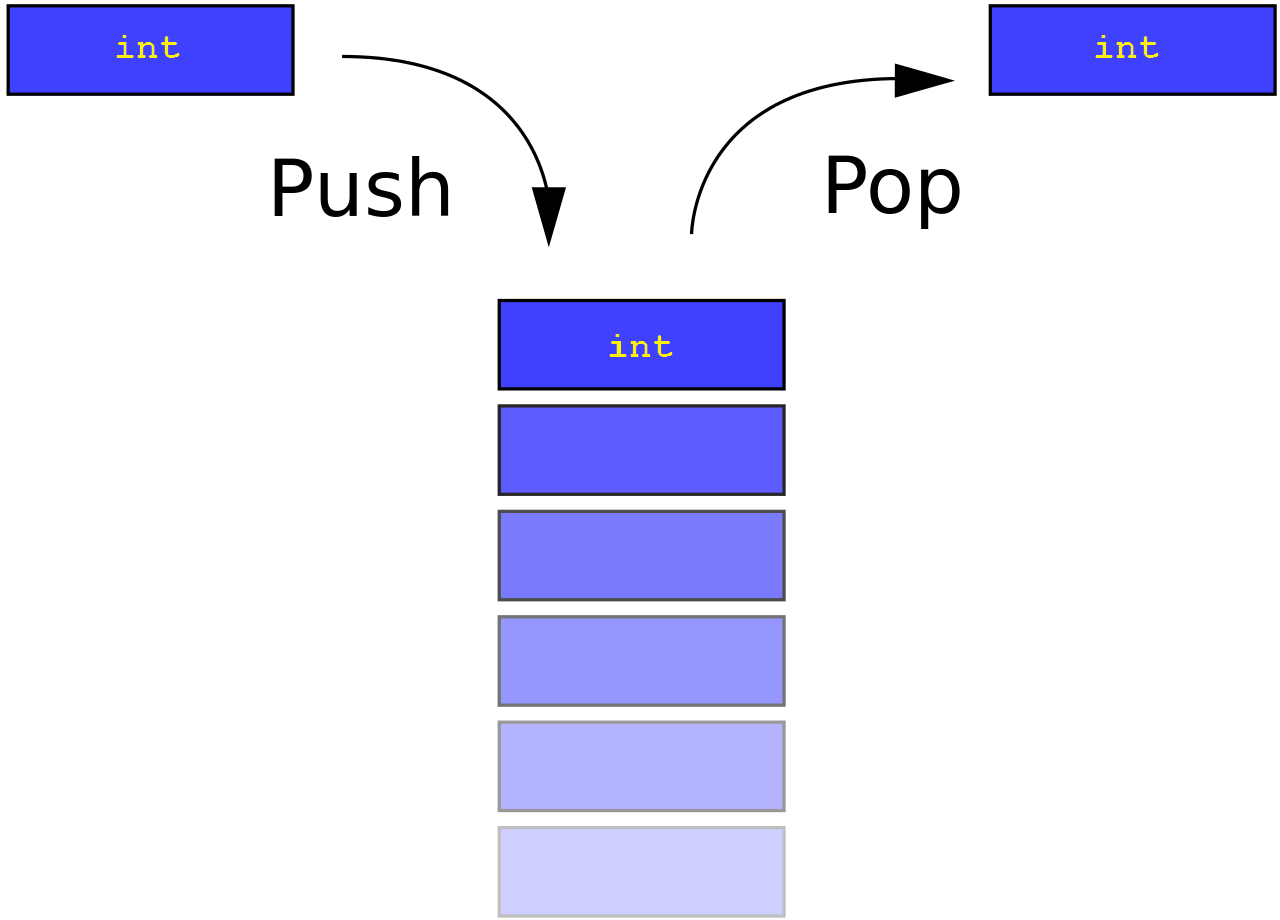
\includegraphics[scale=0.3]{4/stack-int.png}
	\end{center}
\end{document}